\documentclass[a4paper, 11pt, twoside, titlepage]{book}
% Set up page layout
\usepackage[a4paper]{geometry}
\usepackage{fancyhdr}
% Set up hyphenation, etc.
\usepackage[british]{babel}
% Set up images
\usepackage{pstricks,pst-node,pst-text,pst-3d,pst-eucl}
\usepackage{psfrag}
\usepackage{import}
\usepackage{graphicx}
\usepackage{subfigure}
\usepackage[figuresright]{rotating}
%\usepackage{flafter}
% Set up fonts
\usepackage{charter}
\usepackage{amssymb,amstext,amsfonts} %% ... with default font
\usepackage{amsmath}
\usepackage{mathrsfs}
%\usepackage{txfonts}
% Colouring
\usepackage{xcolor}
\definecolor{vermilion}{rgb}{0.80,0.40,}
\definecolor{blueishgreen}{rgb}{0,0.60,0.50}
\definecolor{skyblue}{rgb}{0.35,0.70,0.90}

% Set up lists and tables
\usepackage{listings}
\usepackage{enumitem}
\setlist{itemsep=0pt}
\usepackage{booktabs, longtable, dcolumn,multirow,tablefootnote}
\usepackage{array}
\usepackage{ragged2e}
\newcolumntype{P}[1]{>{\RaggedRight\hspace{0pt}}p{#1}}
\usepackage[labelfont=bf,labelsep=space,hypcap]{caption}
\renewcommand{\captionfont}{\small}
\usepackage[caption2]{ccaption}
%\usepackage{tikz}
%\usetikzlibrary{shapes,arrows}
% More fonts
\usepackage[T1]{fontenc}
\usepackage{lmodern}
\renewcommand{\sfdefault}{lmss}
\renewcommand{\ttdefault}{lmtt}
\usepackage{microtype}
\usepackage[latin9]{inputenc}
\usepackage[11pt]{moresize}
%\usepackage{fixmath}
\usepackage{ upgreek }
% Special symbols
\usepackage{braket}
\usepackage{slashed}
% Set up page indexing, bib fomatting, etc.
\usepackage{afterpage}
\usepackage{appendix}
%\usepackage{paralist}
%\usepackage[linktocpage,bookmarksnumbered,breaklinks,pdfhighlight=/P,citebordercolor=blueishgreen,urlbordercolor=skyblue,linkbordercolor=vermilion]{hyperref}
\usepackage[authoryear]{natbib}
\usepackage[linktocpage,bookmarksnumbered,pdfauthor={Christopher P.L. Berry},pdftitle={Exploring Gravity},pdfkeywords={Ph.D. Dissertation}]{hyperref}            
\usepackage{bookmark}
\usepackage{etoolbox}
% Only link on year
\makeatletter

% Patch case where name and year are separated by aysep
\patchcmd{\NAT@citex}
  {\@citea\NAT@hyper@{%
     \NAT@nmfmt{\NAT@nm}%
     \hyper@natlinkbreak{\NAT@aysep\NAT@spacechar}{\@citeb\@extra@b@citeb}%
     \NAT@date}}
  {\@citea\NAT@nmfmt{\NAT@nm}%
   \NAT@aysep\NAT@spacechar\NAT@hyper@{\NAT@date}}{}{}

% Patch case where name and year are separated by opening bracket
\patchcmd{\NAT@citex}
  {\@citea\NAT@hyper@{%
     \NAT@nmfmt{\NAT@nm}%
     \hyper@natlinkbreak{\NAT@spacechar\NAT@@open\if*#1*\else#1\NAT@spacechar\fi}%
       {\@citeb\@extra@b@citeb}%
     \NAT@date}}
  {\@citea\NAT@nmfmt{\NAT@nm}%
   \NAT@spacechar\NAT@@open\if*#1*\else#1\NAT@spacechar\fi\NAT@hyper@{\NAT@date}}
  {}{}

\makeatother

\renewcommand{\bibfont}{\footnotesize}
\addto{\captionsbritish}{\renewcommand{\bibname}{{R\lowercase{eferences}}}}
%\renewcommand{\refname}{{R\lowercase{eferences}}}
\setlength{\bibhang}{0pt} 
%\setlength{\bibsep}{0.5pt} % 1 linestretch
\setlength{\bibsep}{0pt} % 1.3 linestretch
\addto{\captionsbritish}{\renewcommand{\contentsname}{{C\lowercase{ontents}}}}

%\usepackage{fourier-orns}
  
% Set page layout  
\headheight 13.6pt
% For 10pt text
%\headsep 0.6\baselineskip
%\footskip 2\baselineskip
%\textheight = 55\baselineskip
% For 11pt text
\topmargin -0.4cm
\headsep 0.6\baselineskip
\footskip 2\baselineskip
\textheight = 50.1\baselineskip

\allowdisplaybreaks

% Set numbering depth
\setcounter{secnumdepth}{5}

\def\today{\number\day\space\ifcase\month\or January\or February\or March\or April\or May\or June\or July\or August\or September\or October\or November\or December\fi\space\number\year}

% Custom commands
\newcommand{\eqnref}[1]{equation (\ref{eq:#1})}
\newcommand{\Eqnref}[1]{Equation (\ref{eq:#1})}
\newcommand{\secref}[1]{section \ref{sec:#1}}
\newcommand{\Secref}[1]{Section \ref{sec:#1}}
\newcommand{\chapref}[1]{chapter \ref{ch:#1}}
\newcommand{\Chapref}[1]{Chapter \ref{ch:#1}}
\newcommand{\partref}[1]{part \ref{pt:#1}}
\newcommand{\Partref}[1]{Part \ref{pt:#1}}
\newcommand{\apref}[1]{appendix \ref{ap:#1}}
\newcommand{\Apref}[1]{Appendix \ref{ap:#1}}
\newcommand{\tabref}[1]{table \ref{tab:#1}}
\newcommand{\Tabref}[1]{Table \ref{tab:#1}}
\newcommand{\figref}[1]{figure \ref{fig:#1}}
\newcommand{\Figref}[1]{Figure \ref{fig:#1}}

\newcommand{\units}[1]{\ensuremath{~\mathrm{#1}}}

\newcommand{\sub}[1]{\ensuremath{_\mathrm{#1}}}
\newcommand{\super}[1]{\ensuremath{^\mathrm{#1}}}

\begin{document}

\bibpunct{(}{)}{;}{a}{}{,\,}

\makeatletter
\pagestyle{fancy}
\renewcommand{\sectionmark}[1]{\markright{\thesection\ #1}}
\fancyhf{}
\fancyhead[LE]{Summative assessment}
\fancyhead[RE]{Christopher Berry}
\fancyhead[LO]{FLTHE}
\fancyhead[RO]{\rightmark}
%\fancyhead[RO]{}
\fancyfoot{}
\renewcommand{\footrulewidth}{0.1ex}
\fancyfoot[LO]{\today}
%\fancyfoot[LO]{21st August 2013}
\fancyfoot[RE]{University of Birmingham}
\fancyfoot[RO, LE]{\thepage}
\fancypagestyle{plain}{
\fancyhf{}
\renewcommand{\headrulewidth}{0pt}
\fancyfoot{}
\renewcommand{\footrulewidth}{0.1ex}
\fancyfoot[LO]{\today}
\fancyfoot[RE]{University of Birmingham}
\fancyfoot[RO, LE]{\thepage}}
\makeatother

\frontmatter

\title{{\large\textsc{Foundation of Learning \& Teaching in Higher Education}}\\
\vspace{-5mm}\hrulefill\\
{\Huge\textsc{Tutoring Second-Year Physics\\\& Key Skills}}\\
\vspace{-2mm}\hrulefill\\
\vspace{-2mm}{\large\textsc{Postgraduate Certificate in Academic Practice}}}

\author{{\Large{}Christopher Berry}\\
\vspace{1mm}\href{mailto:cplb@star.sr.bham.ac.uk}{cplb@star.sr.bham.ac.uk}\\
\vspace{1mm}School of Physics \& Astronomy}

\date{\today} 

\maketitle

\tableofcontents

\mainmatter

\chapter{Overview}

In this work we examine the small-group teaching of second-year physics undergraduates. This teaching takes the form of regular tutorials. The role of small-group tutorials (SGTs) within physics is introduced in \chapref{intro}.\footnote{In the context of teaching physics, we consider a small group to be one consisting of 2--6 students, which follows \citet[chapter 1]{Jaques2007}. My own groups range in size between 2 and 5 students.} Here, I reflect upon my own educational experiences as well as research on teaching and learning \citep{McCarthy2008}. One of the components of tutorials is the teaching of key skills: compiling a curriculum vit\ae{} (CV), giving a presentation and writing an essay. These transferable skills are valuable assets when the students graduate and seek employment \citep{Pike2015}. Teaching these communication skills is different from the more familiar teaching of subject material and so I have chosen to examine my practices in more detail, concentrating on essay writing. In \chapref{essay} I discuss a plan for this teaching, I introduce a new elements to my delivery, a formative essay designed to give feedback \citep[feedforward;][]{Bloxham2015} and practice, and blog posts that can be referred to outside of tutorial.\footnote{The posts can be read at \url{http://cplberry.com/tag/writing/}.} In \chapref{conc}, I evaluate their impact. In the process of this, I draw upon feedback from students (\apref{student}) and peers (\apref{peer}), my own training (e.g., \apref{Scriptoria}), and the final marks (\apref{marks}). I find that the formative essay has a small positive effect on the achievement of my students, but this impact could potentially be improved by adapting its format; as might be expected, the students' motivation and proficiency remain the dominant predictors of their essay-writing ability \citep{Ketteridge2015}.


\chapter{Introduction to tutoring physics}\label{ch:intro}

In this chapter we discuss the teaching and learning of physics with particular reference to my experiences. We learn from our own experiences, repeating things that have gone well, and avoiding those that led to failure \citep[chapter 2]{Skinner1954,Kolb1984}. When reflecting upon our teaching, we must consider how our perception is influenced by personal experience, and how our students may not share the same view;\footnote{The Johari window gives a simple way of visualising how one's own experience does not overlap with others', but one's outlook can be expanded through feedback \citep{Luft1961}. Sharing experiences (exposing one's own knowledge) with others can be considered an aspect of teaching \citep[cf.][chapter 7]{Ramsden1992}.} hence, we begin with a brief summary of my personal development in \secref{teach-n-learn}. From here we introduce core components of studying physics (\secref{physics}), before expanding upon small-group teaching (\secref{small}), a primary element of both my learning and teaching experience. %Building upon the ideas of learning in a small group, my experiences of learning through peer collaboration are discussed in \secref{peer}.
The chapter concludes with a critique of how I have assimilated aspects of my student experience into my approach to teaching.

\section{Teaching \& learning}\label{sec:teach-n-learn}

My own teaching style reflects how I learnt as I attempt to emulate those experiences most educational for me. Since I was both sufficiently academically able and interested in my subject to continue to a research position, it may be assumed that I do not reflect the average student. While my experience is a sensible starting point, it is vital to remember that others may have different preferences \citep[chapter 5]{Ramsden1992} and those who need the most support will be those who find the subject more difficult. To try to understand other perspectives and broaden my outlook, it is necessary to seek feedback (see appendices \ref{ap:student} and \ref{ap:peer}) and research studies of educational practices (discussed throughout).

I read Natural Sciences (Experimental \& Theoretical Physics) at the University of Cambridge as an undergraduate, before continuing to complete a Ph.D.\ in Astronomy. During my postgraduate study I began supervising: tutoring small groups (2--3 students), with teaching focussed on weekly (formative) problem sets. These had been an integral part of my undergraduate study, hence I was familiar with their function and form. Following completion of my doctorate, I have moved to the University of Birmingham, where I now tutor: small-group (3--5 students) teaching similar to supervising, except that problems also play a summative role. At both Cambridge and Birmingham, I have taught second-year physics for these SGTs.

This academic year, I have continued my personal development by lecturing a short, optional course to a mix of fourth-year undergraduates and postgraduate students.\footnote{The course was approximately $52\%$ undergraduates, $34\%$ postgraduates and $14\%$ interested staff.} Lecturing is not discussed in detail in this work, but there are many parallels between SGTs and lectures (see \secref{other}): explaining clearly; maintaining an environment suitable for learning; checking students' understanding and progress; planning material to deliver and doing so at good pace (within a fixed time); engaging students in discussions and interesting them in their studies, and seeking feedback from students (\citealt[chapter 3]{Brown1988}; cf.\ \citealt[chapter 6]{Ramsden1992}).\footnote{Tutorials can become too much like lectures \citep[chapter 9]{Ramsden1992}; in a study of SGTs in British universities, \citet[quoted in \citealt{Brown1988}, chapter 4]{Luker1987} found that between $7\%$ and $70\%$ of time is spent by the tutor lecturing.} My experience with SGTs made it more natural for me to engage with the class and have them work through problems, which proved popular. I was surprised at how difficult it was to judge the time to cover a particular topic. I am used to going through problems and explaining concepts in tutorials, and keeping to an hour time-slot; however, extending this to a lecture where a single narrative, explained such that a large group can keep up, must be contained within a hour was challenging. This has made me more conscious of how I allocate time in tutorials, and in particular that I leave time for a summary at the end to recap what we have discussed.\footnote{The usefulness of an ending summary was highlighted through my experience of peer observations (both reflecting on feedback on my tutorials and while observing the lecturing of another) discussed in \apref{peer}.}

\section{Studying physics}\label{sec:physics}

Physics is a broad subject covering the fundamental behaviour of the Universe and its components. Familiar to most as it is introduced at school level, its teaching follows a spiral curriculum, periodically returning to previously-taught topics to cover them in ever-expanding detail \citep{Bruner1960}. The main jump from school to university physics is in the use of mathematics. Applying mathematical formalism to describe and solve physical problems is the greatest threshold concept \citep{Meyer2003} faced by those wishing to become conversant with physics \citep{Wigner1960,Roth1994}.

My experience of university-level physics teaching has been traditional \citep[cf.][]{Iannone2015}. Concepts and theories are introduced in lectures, and reinforced through problem sets that also encourage mathematical fluency and independent learning \citep{Pike2015}. Some of these problems are assessed to provide students with feedforward information \citep{Bloxham2015}. SGTs or examples classes give students the opportunity to discuss the problems and their solutions, as well as other elements of the syllabus.\footnote{This may fulfil the role of inverted classrooms, where students prepare outside of class and then work through problems under the guidance of a tutor in class, employed elsewhere \citep{Lage2000}.} Practical work is done in labs; experiments may complement topics covered in lectures; % for example measuring refraction during a course on electromagnetism;
be of equal importance as lectures for teaching ideas, %for example in a course on electronics,
or motivate material covered in lectures %, for example error analysis
\citep{Hanif2009}. Assessment is dominated by summative closed-book examinations at the end of the courses.\footnote{The situation may be comparable to that in mathematics where traditional closed-book examinations are favoured \citep{Iannone2014}, as both subjects require similar (mathematical) problem solving and the correctness of solutions is not subjective.} I have found completing problem sets best encourages deep learning \citep{Marton1976,Marton1976a}: good understanding is required to fully solve a question and, since problems are done outside of class, there is sufficient time to review and assimilate new ideas (see \secref{tutorial-value}).\footnote{Even if a student takes an achieving strategy \citep[chapter 2]{Biggs1987} and only invests time in understanding the topics directly probed by the given questions, a dense covering of the syllabus by problems sets should ensure a comprehensive understanding of the majority of the material.}

Problem sets are of paramount importance, both for teaching subject material and key skills such as problem solving and mathematical proficiency. Extracting the most from them relies on the student being motivated to put in the necessary effort: those who work harder shall learn more \citep{Gibbs2015}. This is difficult to externally inspire \citep[cf.][]{Ryan2000}, especially since a student taking a surface-learning approach is more likely to find problems tedious and unprofitable, potentially pushing them further away from engaging with the material \citep[chapter 4]{Ramsden1992}. Consequently, we shall instead focus on how problem sets are supported, which is primarily through SGTs.

\section{Small-group teaching}\label{sec:small}

Supervisions at Cambridge involve either an academic or a Ph.D.\ student meeting regularly with a group of students. The small group size allows for sessions to be tailored to the individual needs of the students and for each student to be involved in discussions.\footnote{Groups of only one student are usually avoided as this could be intimidating for the student. Furthermore, having an additional student provides some respite to think while the other is being questioned. The lone student would also miss out on the opportunity to hear the opinions of a peer.} Supervisions are generally structured around the problems, with the students given opportunity to ask about other areas of the course they were unsure of (or interested in); any spare time is used to discuss additional topics. The supervision system is designed to encourage students to stay on top of their work and to provide them with the necessary support when this is difficult; the overall effect is to promote deep learning \citep[case study 14.1]{Gibbs2015}.

Tutorials in Birmingham are of a similar nature to supervisions. They differ in group size, which does not afford as intensive attention to individuals, and in the amount of contact time. In second year, Cambridge's Natural Sciences undergraduates would have three hours per week (one per course), while Birmingham's Physics undergraduates have a single hour per week for all their courses.\footnote{The difference in teaching time is slightly ameliorated by the marginally longer teaching year in Birmingham: 22 weeks compared to 19.} While the tutorial system might not match supervisions in Cambridge, they still provide a great opportunity for students to engage with and ask questions of a member of research staff, an opportunity that is not present in all courses.\footnote{\citet{Sharma2007} notes how SGTs are of particular importance to physics students, with the interactivity and development of problem-solving skills praised, but that they are not present at all institutions through all years of study.}

A further difference is that tutorials in Birmingham include the (formal) teaching of key communication skills. These are part of the curriculum at Cambridge, but not explicitly taught in supervisions. %(although students are still at liberty to ask about these topics).
I believe that teaching of these soft skills is to be encouraged as they are of universal utility and a necessity for employment; one of the objectives of higher education should be to prepare students for life and world outside of study \citep{Fallows2000,Harvey2000}. Communication skills enhance the employability of the students; they are not traditionally emphasised within a physics course \citep[cf.][]{Sharma2007}, but are considered a key area of competency for a physicist \citep{Gonsalves2014a}. However, including teaching of communication skills in tutorials also absorbs time that could have been spent on the main curriculum, further limiting the time for discussing problem sets or lecture material. Striking a balance between different aspects of the curriculum is difficult.

%For any SGT it is necessary for students to prepare. I did this by collaborating with my peers. Cooperative learning encourages learning in physics \citep{Springer1999,Crouch2001,Pilzer2001,Miller2006} and gives practice explaining physics.

%\section{Peer learning}\label{sec:peer}

%As an undergraduate, I would often work on problems with a group of fellow physicists. Doing so provided support for difficult questions, an opportunity to discuss concepts, and multiple points-of-view. It made the experience much more enjoyable, and motivated continued effort \citep[e.g.,][chapter 1]{Roth1994,Springer1999,Falchikov2001}: working on questions was a social activity, and there was friendly competition to finding (the best) solutions. Cooperative learning has been found to improve student attainment (\citealt{Qin1995}; \citealt[chapter 2]{Falchikov2001}; \citealt{Cabrera2002}), and this particular example can be considered as an informal version of peer instruction \citep{Roth1994}, which has been demonstrated to be effective in encouraging learning in physics \citep{Springer1999,Crouch2001,Pilzer2001,Miller2006} and deep learning in general \citep{Marton1976,Wilson2005}.
 

\section{Translation from learning to teaching}

Several elements from my own studies have been incorporated into my current teaching style. From Cambridge I have inherited high expectations for my students' work. This helps stretch them to achieve their best, and engage them by challenging them academically \citep{Bamber2015}. I explain my expectations with students during our first meeting (see \apref{plan}) to make sure these are explicit \citep{Butcher2015}, and to try to ensure that the students appreciate the standards required of them \citep[chapter 8]{Ramsden1992}. Many students have expressed approval of having high targets set, either because they are eager to be challenged or because they like to have clear goals to motivate themselves; of course, this does not translate to students always being adequately prepared for tutorials; usually there is a decline as the term progresses and students become fatigued or over-burdened with work (see \secref{timetable}).

In my SGTs, engaging students in conversation is important: they need to actively discuss concepts, and ask questions freely. Cambridge gave me much experience of discussing physics, both in supervisions and working outside, and I believe this has greatly benefited my teaching (see sections \ref{sec:A-topic} and \ref{sec:B-topic}).

Having now established some of the core components of undergraduate physics education and discussed how my own education has influenced my teaching, we will move on to look at specific aspects of my SGTs, and how these are designed and evaluated.


\chapter{Teaching essay writing}\label{ch:essay}

In this chapter we shall examine in detail my teaching of essay writing. SGTs have been my primary experience of teaching (\secref{teach-n-learn}) and are an important component of an undergraduate physics course (\secref{small}) making them the natural subject for me to study my teaching. There are many aspects of tutorials, too many to examine in detail. The teaching of communication skills is one aspect that differs between my previous teaching in Cambridge and my current teaching in Birmingham. I have therefore selected essay writing, one component of this, as a subject. Conclusions drawn from how I teach essay writing should transfer to the teaching of other parts of the curriculum in tutorials.

We begin with a description of essay writing within the second-year course in \secref{problem}. Then we look at how I teach essay writing in \secref{essay-teach}. I discuss my approach across both years of giving tutorials. I was dissatisfied with the effectiveness of my teaching in the first year, in particular I was concerned that some topics such as referencing, although covered in detail, but remained problematic. I identified, with help from peer discussion (\secref{ALS}), several areas where teaching could be enhanced, and decided to introduce two new elements to my teaching: setting a formative, practice essay and providing written advice that can be used as reference. These are described in sections \ref{sec:formative} and \ref{sec:blog} respectively. The outcomes of my teaching are evaluated in \chapref{conc}.

\section{The second-year essay}\label{sec:problem}

Second-year Physics students at the University of Birmingham must write an essay as part of their (compulsory) Physics \& Communication Skills 2 module, constituting $10\%$ of the marks for the module, which in turn makes up $10$ out of $120$ credits for the year. This means the essay is worth just under $1\%$ of the students' second-year grade. Students will have previously written an essay in their first year as part of their skills training; this makes up $15\%$ of a $10$ credit module and shares an identical mark scheme to the second-year essay. The essay assessment emphasises writing proficiency over scientific content; the mark scheme is described in \tabref{mark-scheme}.\footnote{Taken from the Year 2 Physics and Communication Skills handbook \url{https://intranet.birmingham.ac.uk/eps/documents/staff/physics/students/handbook/handbook-y2-comms.pdf}.}
\begin{table}\scriptsize
\centering
\begin{tabular}{c c p{3in}}
\toprule
\multicolumn{1}{c}{Mark subsection} & \multicolumn{1}{c}{Category} & \multicolumn{1}{c}{Description} \\
\midrule 
\multirow{4}{*}{Content} & \multirow{1}{*}{Topic}  & Conceptually challenging and well treated $\leftrightarrow$ Inappropriate and poorly treated \\
			 & Reading	  & Wide range of source material $\leftrightarrow$ Little evidence of research \\
			 & Understanding  & Clear grasp of material $\leftrightarrow$ Uncritical rehash \\
\midrule
\multirow{9}{*}{Style}	 & Structure 	  & Introduction, development of topic and conclusion. \\
			 & English  	  & Grammar, paragraphs, sentences, spelling, etc. \\
			 & Basic writing style  & Mature, rigorous and scientific. \\
			 & \multirow{1}{*}{Clarity}  & Logical development, appropriate level, definition of terms, etc. \\
			 & \multirow{1}{*}{Presentation}  & Standard of word processing/typographical errors/layout of title, fonts and diagrams. \\
			 & \multirow{1}{*}{Referencing}  & Appropriate referencing of paper and electronic sources, including figures. \\
\midrule
\multirow{1}{*}{Discretionary}	 & Overall impression & --- \\
 \bottomrule
\end{tabular}
\caption{Mark scheme for the (first- and) second-year essay. Each category is worth $10$ marks, giving a total of $100$. The emphasis is on good scientific writing ($60\%$ of the marks) rather than on scientific content ($30\%$). Being outside of the word limits results in a loss of $10\%$ from the mark, and late submission results in a penalty of $10\%$ per day. Students who score below $60\%$ have to resubmit a revised version within two weeks; failure to do so results in a score of zero. Resubmitted essays are capped at a maximum mark of $60$.}\label{tab:mark-scheme}
\end{table}

The essay can be on any physics-related topic (except those used for the first-year essay and their oral presentation). The students must research this themselves. The word limit is $2000 \pm 200$. 

In addition to the essay, students have other pieces of assessed, extended scientific writing associated with their projects (another $10$ credit module). They must write a preliminary report of $2$--$4$ sides of A4 by the third week of the Spring Term (see \apref{plan}). This is worth worth $10\%$ of the module and its main purpose is to ensure that students have a plan for their projects. Accordingly, written style is not too important provided that students can produce a concise and technical report. Following completion of their essay, they have to submit a write-up of their project. This report has a maximum length of $20$ sides of A4 and is worth $50\%$ of the module. Marks are awarded both for the quality of the project (judged from the report) and quality of the report itself. This project report is both longer and worth more marks than the essay, hence using the essay as a means of improving scientific writing is beneficial for the student. The essay must be submitted by the end of week 6 of the Spring Term (see \apref{plan}) and the project report by the end of week 11; this gives a short time to receive and digest feedback from the essay, making it advantageous for students to receive guidance and to think about their writing style earlier in the year.


\section{Teaching plan}\label{sec:essay-teach}

In this section we discuss my teaching of essay writing, beginning with a description of some of the key learning outcomes I have identified (\secref{essay-aims}). Then we discuss how the essay fits into the schedule for tutorials (\secref{timetable}) and some of my specific approaches to teaching (\secref{essay-methods}). I discuss my teaching both last year (\secref{teach2013-14}) and this year (\secref{teach2014-15}) and highlight two new aspects (sections \ref{sec:formative} and \ref{sec:blog}).

\subsection{Objectives}\label{sec:essay-aims}

Scientific writing (as an essay, report or paper) has many aspects, as indicated in \tabref{mark-scheme}. Most fundamental is the ability to communicate clearly using English properly. It should be assumed that students have a basic proficiency with written English before they start university; in practice, English levels may not be as high as is desirable, particularly for international students who are not native speakers and understandably find it more difficult. Support for improving written English is available from the Academic Skills Centre,\footnote{The Academic Skills Centre is run by the University of Birmingham Library Services \url{https://intranet.birmingham.ac.uk/as/libraryservices/library/skills/asc/index.aspx}} and English-language support for international students is available from the English for International Students Unit.\footnote{The English for International Students Unit is part of the University of Birmingham's Academic Services \url{https://intranet.birmingham.ac.uk/as/eisu/insessional/index.aspx}} In my tutorials I will focus on aspects of academic, scientific writing that are different from less formal writing and so are less familiar.

I will split the differences between scientific writing and more general written English into three classes:
\begin{enumerate}
\item Specialisations---Modifications of familiar concepts to match the expectations of formal scientific writing, e.g.\ the structure of an introduction, main body and conclusion.
\item Conventions---Rules for particular aspects of the writing that may be simple to follow, but could be overlooked if not explained, e.g.\ the proper typesetting of mathematics.
\item Threshold concepts \citep{Meyer2003}---The most challenging ideas to grasp as they require a transformation of how the work is viewed, e.g.\ the need for referencing.
\end{enumerate}
The first is easiest to teach and the third is most difficult, although all three are important and require attention. Specialisations include adopting an appropriate structure, using a formal tone and scientific language (aspects of the Structure, Basic writing style and Clarity mark-scheme categories). Many of these concepts may be familiar and students may just need to extend their current practices. Conventions are often arbitrary and may not be immediately apparent to the uninitiated, such as the distinction between italic and roman (upright) typesetting of terms in equations, how to label graph axes, or how to format entries in a bibliography. These primarily fall under the heading of Presentation in the mark scheme; following them makes the writing more recognisable as a piece of scientific text. Once students are aware of the conventions, following the rules is not challenging, but it may be difficult to convince the students that this is worth the effort. Threshold concepts are the ideas that have the largest impact on the development of the students and are discussed further in \apref{threshold}. For my students, I have found three threshold concepts:
\begin{enumerate}
\item Not restricting themselves to prose---Using equations, diagrams or graphs, tables or even bullet points to communicate information (depending upon the audience).
\item Referencing \citep{Warner2011}---Including in-text citations to appropriate sources in the relevant places to support and supplement their arguments.
\item Being quantitative---Using numbers (either empirical or theoretical) to make specific quantitative statements, either to replace potentially subjective qualitative statements or to provide unambiguous evidence for a statement, e.g. saying ``the surface of the Sun is $6000~\mathrm{K}$'' rather than ``the surface of the Sun is hot''.\footnote{Both a cup of tea and the centre of the Sun could equally be claimed to be hot but both have temperatures that are orders of magnitude different from the surface of the Sun. The lack of quantitative statements could be viewed as the surface manifestation of a deeper problem of failing to understand that a reader who wants to engage with the material, to evaluate the validity of the arguments or to perform their own calculations, would require this information.}
\end{enumerate}
Identifying means to make learning these concepts easier could potentially have a significant impact on the quality of students' written work.

\subsection{Scheduling}\label{sec:timetable}

Given infinite time, all of the previous subsection's concepts could be perfectly taught. However, tutorials are finite and must cover more than writing skills (\secref{small}). In \apref{plan} there is an outline for tutorials through the year. Students must not be over-burdened as this is detrimental to their learning \citep[chapter 8]{Ramsden1992}, and a perceived heavy workload is correlated with adoption of a surface-learning approach\citep[and references therein]{Kember1998}.\footnote{\citet{Kember1998} find the workload is perceived as higher by students learning in a second language, which makes it especially important not to schedule too much for international students.}

In the Autumn term, students must prepare oral presentations (also worth $10\%$ of the Physics \& Communication Skills 2 module), which must be delivered by the end of the term. This leaves little time for written communication skills. However, it is possible to link the two types of communication skills together: there is significant overlap between the two (thinking of audience, planning structure, presenting technical content, conducting research, etc.). Thus, preparing and delivering the presentation can be used as instruction for the essay provided that the connections are made apparent. This integration has the additional benefit of ensuring that the presentation is not viewed as an isolated task, encouraging students to use feedback from this experience \citep{Housell2003}.

Following completion of the presentations, students have the Christmas vacation and the first half of the Spring term for their essays. The vacation provides a good opportunity to pick a topic and begin research, and writing skills can be discussed when they return. The Spring tutorials will be where most of the teaching is done.

While the presentation precludes spending time of writing skills for much of the Autumn term, there remains some freedom at the start of the year. In the first few weeks, students' workloads are lower, since problem sets have yet to be issued, and consequently there is less to be discussed during tutorials. Students do have to provide an updated CV by the third tutorial of term, but this is a small task that can be accomplished quickly.\footnote{The students write a CV in first year, so it only requires a few modifications to bring it up to date. Discussing their CV in the first one-on-one meeting is a useful way to get to know the students and it leads naturally onto their academic background, how they did last year, and where they hope to be in the future.} This time at the start of the year could potentially be filled with material relating to the essay.

\subsection{Methods \& activities}\label{sec:essay-methods}

\subsubsection{Tutorials \& feedback}

Teaching of essay writing has followed a similar design to any other curriculum item. I discuss items with the students to keep pace with their work, and work through examples on the board. They are free to ask questions and suggest topics that require particular attention. I suggest other sources of information or useful activities for outside of tutorials, and draw connections to other areas of the syllabus. Following completion of the work, I provide feedback and we discuss troublesome areas.

My own experience of being taught writing skills follows a similar pattern, as detailed in \apref{Scriptoria}.

During discussions, specialisations arise naturally. Students know that these are things to ask about and potentially develop further. Proximal zone. Following initial questions, I cover any elements they had not thought of. This leads naturally into me bringing up conventions as I can highlight them as something they are probably unaware of. Working through some model answers, is intended to help them to assimilate this knowledge \citep[chapter 10]{Ramsden1992}. Larger topics (threshold concepts) require more attention and detailed explanations planned ahead of the tutorial.

Following submission, I try to provide detailed feedback that students could use. For each student, I ensure there is one aspect that was given specific praise\citep{Henderlong2002}. Together with their mark for each category (\tabref{mark-scheme}) I give comments highlighting good areas and those for improvement. On the essays themselves I give detailed comments, highlighting good and bad practices, using two different colours: one colour for smaller matters such as spelling or typographical errors, which are not normally considered important feedback \citep[chapter 4]{Irons2008} but are emphasised in this mark scheme, and another colour for the more complex issues, such as comments on physics, logical development or essay structure. The feedback is discussed at length in tutorial, where specific examples are examined and students can ask questions \citep[chapter 2]{Irons2008}.

\subsubsection{2013/2014}\label{sec:teach2013-14}

The first year I gave tutorials, my essay preparation consisted of three main components (\tabref{2013-14}): asking the students to begin researching and planning their essay over Christmas, to be discussed in the first week of term; a main discussion of scientific writing with special emphasis on referencing, which they had highlighted as an area of concern (see \apref{threshold}), in the third week of term, and a final session to recap points I had made earlier (in particular, expand on conventions) and to ensure that students are familiar with the mark scheme (\citealt[chapter 8]{Ramsden1992}; \citealt{Bell2012}) in the fifth week of term. These three sessions can be seen to roughly align with the three stages of essay construction proposed by \citet{Biggs1988}: intentional (establishing aspirations prior to writing), parawriting (planning and updating knowledge), and writing (composing, reviewing and revising).

To try to make the assessment less stressful \citep[chapter 10]{Ramsden1992}, I offered office hours for any last minute problems or questions to be discussed one-on-one. Additionally, I suggested students handed in their essay to me a day early, such that there was time to correct any common, trivial mistakes (such as forgetting the word count or missing a page) and subsequently have time to grapple with any technical problems of submitting electronically.

I was slow in delivering feedback, which is suboptimal \citep[chapter 4, and references therein]{Irons2008}, providing it in week 10. This was not only disadvantageous for the students to learn from the assessment, but also meant that it would be difficult for them to incorporate feedback into the writing of their project report. Furthermore, I had not anticipated that any students would need to resubmit an essay, yet this was the case, and had to be done during the Easter vacation when it was not easy for them to talk to me.

\subsubsection{2014/2015}\label{sec:teach2014-15}

This academic year, I made several changes to my teaching (\tabref{2014-15}). First, I introduced a formative essay. The discussion following this, pre-empted much of the material presented in the twelfth 2013/2014 tutorial. In the equivalent tutorial this year, we recapped these points briefly before spending more time on the threshold concepts (primarily referencing). The discussion spilled over into the next tutorial, where the conventions of presenting mathematics were explained, which also gave a chance to link with the concept of including equations in the text. Although the tutorial discussions have been expanded and spread throughout the year, their character has not changed.

Feedback was provided more promptly \citep{Gibbs2015}. This should give it more impact and make it more likely to be assimilated as it becomes feedforward for the project report \citep{Housell2003,Bloxham2015}.

\subsubsection{Formative essay}\label{sec:formative}

In 2013/2014, following feedback discussions, several students expressed regret that they had not appreciated concepts prior to assessment. This led naturally to the idea of setting a formative essay and providing feedback on this earlier in the year. Formative assessments have many advantages: students are more likely to be open with their concerns; experiment and take risks; be motivated by their own learning, and develop their self-assessment \citep[chapter 1, and references therein]{Irons2008}, additionally, they can help establish expected standards \citep[chapter 10]{Ramsden1992}. The practice essay also gives me opportunity to diagnose troublesome issues.

The main barrier to introducing a formative essay was the additional work \citep[chapter 4]{Irons2008}. Given time-table constraints (\secref{timetable}), the only gap was at the start of the year. I asked the students to produce a short essay on any topic such that they did not have to worry about research, and could concentrate on writing.\footnote{I specified that they must still include references.} The disadvantage of an early formative assignment was the disconnect from the summative one. The solution was to link writing skills with presentation skills: the formative essay feeds into the presentation which then feeds into the summative essay (which feeds into the project report). Teaching of communication skills is distributed throughout the entire year, with no gaps where they become irrelevant.

I provided (prompt) feedback on the formative essay as I would for the summative essay except I did not give marks \ldots. This was then discussed in tutorial where I also highlighted my blog as a useful reference for the material we discussed.

\subsubsection{Written resources}\label{sec:blog}

To complement the feedback from the formative essay, I produced a blog post containing advice and examples \citep[chapter 4]{Irons2008}.\footnote{This is also time-efficient for me, as the same advice can be recycled for multiple years \citep[chapter 4]{Irons2008}.} This can be read at \url{http://cplberry.com/right-good/}. It can be used as a reference following the tutorial and I hoped students would refer to it when writing (see \apref{Scriptoria}). The possibility to review and ask questions (via comments) within their own time can help students, particularly non-native speakers, absorb the material \citep{Rainsbury2003}.

The blog post was well-received (\secref{me}), so I composed a second on the conventions of typesetting mathematics to reinforce the material from the thirteenth tutorial (\apref{plan}). This can be read at \url{http://cplberry.com/right-good/}. Providing a single, easy-to-find reference for conventions, specifically designed for these students, should assist their learning \citep[cf.][chapter 9]{Ramsden1992}; the effectiveness of the blog is reviewed in the next chapter.



\chapter{Evaluation \& conclusions}


\appendix
\chapter{Teaching plan}\label{ap:plan}

Tutorials are primarily focussed upon topics the students are having difficulty with or are particularly interested in learning more about. On a week-by-week basis, I plan the contents of tutorials around problem sets. I always leave time for students to raise topics and to discuss what they have been covering in lectures. Around these activities, I must schedule the teaching of key skills (CV preparation, giving a presentation, writing an essay and revision). Below I give my macroscale plan for tutorials that includes when significant elements of the key-skills course components are covered, but not the smaller details of which problems or lectures would be covered in each session.

The tutorial plan for the 2013/2014 academic year is shown in \tabref{2013-14}, and the plan for 2014/2015 is shown in \tabref{2014-15}. The most significant difference between the two is the introduction of a practise essay. The plan lists the plan for twenty tutorials across the autumn and spring terms plus one revision tutorial in the summer term. One of the tutorials in the autumn term is replaced by a careers tutorial; this is delivered by a member of the careers service and is subject to their time-constraints. In addition to the regular tutorials, there are one-on-one meetings at the start of the year, which serve as an introduction, and half-way through the year, which are progress review tutorials (PRTs). I use the PRTs to not only give feedback on the students' performances, but also to ask for feedback on mine. Also included in the plans are the dates of the essay deadline (both the final deadline and the early deadline I set in order to prevent last-minute panic) and the time that I make available as office hours should any students wish to talk about their essay. These plans are discussed in \ldots

\begin{table}\scriptsize
\centering
\begin{tabular}{c c r c l l}
\toprule
\multicolumn{1}{c}{Term} & \multicolumn{1}{c}{Week} & \multicolumn{1}{c}{Date} & \multicolumn{1}{c}{Activity} & \multicolumn{1}{c}{Work} & \multicolumn{1}{c}{Topic} \\
\midrule 
\multirow{11}{*}{Autumn} & \hphantom{0}1 &	 2/10/2013 & 1-on-1		& Draft CV		& Mention key skills and discuss CV \\
			 & \hphantom{0}2 &	 8/10/2013 & 1st		& CV			& \\
			 & \hphantom{0}3 &	15/10/2013 & 2nd		& 			& Introduce presentations \\
			 & \hphantom{0}4 &	22/10/2013 & 3rd		& Talk idea		& \\
			 & \hphantom{0}5 &	29/10/2013 & Careers		& 			& \\
			 & \hphantom{0}6 &	 5/11/2013 & 4th		& Talk outline		& How to give a talk \\
			 & \hphantom{0}7 &	12/11/2013 & 5th		&			& \\
			 & \hphantom{0}8 &	19/11/2013 & 6th		& Talk draft		& Talk content and structure \\
			 & \hphantom{0}9 &	26/11/2013 & 7th		&			& Presentation assessment criteria \\
			 & 10		 &	 3/12/2013 & 8th		& Presentations		& \\
			 & 11 		 &	10/12/2013 & 9th		&			& Presentation feedback \\
\midrule
\multirow{15}{*}{Spring} & \hphantom{0}1 &	17/01/2014 & 10th		& Essay idea		& \\
			 & \hphantom{0}2 &	24/01/2014 & 11th		&			& \\
			 & \hphantom{0}2 &	24/01/2014 & PRT		&			& \\
			 & \hphantom{0}3 &	31/01/2014 & 12th		&			& Academic writing and referencing \\
			 & \hphantom{0}4 &	 7/02/2014 & 13th		&			& \\
			 & \hphantom{0}5 &	14/02/2014 & 14th		&			& Essay advice and marking criteria \\
			 & \hphantom{0}6 &	19/02/2014 & Office hours	&			& \\
			 & \hphantom{0}6 &	20/02/2014 & Early deadline	& Finished essay	& \\
			 & \hphantom{0}6 &	21/02/2014 & 15th		&			& \\
			 & \hphantom{0}6 &	21/02/2014 & Final deadline 	& Finished essay	& \\
			 & \hphantom{0}7 &	26/02/2014 & 16th		&			& \\
			 & \hphantom{0}8 &	 7/03/2014 & 17th		&			& \\
			 & \hphantom{0}9 &	14/03/2014 & 18th		&			& \\
			 & 10		 &	21/03/2014 & 19th		&			& Essay feedback \\
			 & 11		 &	28/03/2014 & 20th		&			& Revision and past-papers \\
\midrule
\multirow{1}{*}{Easter} & \multicolumn{1}{c}{---} & 4/04/2014 & Essay resubmission & Revised essay	& \\
\midrule
\multirow{1}{*}{Summer}	 & \hphantom{0}1 &	 1/05/2014 & Revision		&			& \\
 \bottomrule
\end{tabular}
\caption{Tutorial teaching plan for the academic year 2013/2014. Teaching activities are listed by term, week number and date. Included are twenty regular tutorials, one revision tutorial and a careers tutorial (delivered by the careers service). In addition to these, is the one-on-one (1-on-1) meeting at the start of the year, which serves as to introduce student and tutor, and the progress review tutorial (PRT) at the start of the second term. The dates of the essay deadlines and the office hours for discussion of essay writing are also included. The penultimate column lists task or pieces of work that the student is expected to complete and bring along. The final column lists topics pertaining to key skills that are discussed in detail, this does not include brief checks of progress, quick questions from students, etc.}\label{tab:2013-14}
\end{table}

\begin{table}\scriptsize
\centering
\begin{tabular}{c c r c l l}
\toprule
\multicolumn{1}{c}{Term} & \multicolumn{1}{c}{Week} & \multicolumn{1}{c}{Date} & \multicolumn{1}{c}{Activity} & \multicolumn{1}{c}{Work} & \multicolumn{1}{c}{Topic} \\
\midrule 
\multirow{11}{*}{Autumn} & \hphantom{0}1 &	 2/10/2014 & 1-on-1		& Draft CV		& Mention key skills and discuss CV \\
			 & \hphantom{0}2 &	 9/10/2014 & 1st		& CV			& Set essay \\
			 & \hphantom{0}3 &	16/10/2013 & 2nd		& Formative essay	& \\
			 & \hphantom{0}4 &	23/10/2013 & Careers		& 			& Introduce presentations \\
			 & \hphantom{0}5 &	30/10/2013 & 3rd		& 			& Essay feedback \\
			 & \hphantom{0}6 &	 6/11/2013 & 4th		& Talk idea		& Presentation assessment criteria \\
			 & \hphantom{0}7 &	13/11/2013 & 5th		& Talk outline		& \\
			 & \hphantom{0}8 &	18/11/2013 & 6th		& 			& How to give a talk \\
			 & \hphantom{0}9 &	27/11/2013 & 7th		& Talk draft		& Talk content and structure \\
			 & 10		 &	 4/12/2013 & 8th		& Presentations		& \\
			 & 11 		 &	11/12/2013 & 9th		&			& Presentation feedback \\
\midrule
\multirow{15}{*}{Spring} & \hphantom{0}1 &	12/01/2014 & 10th		& Essay idea		& \\
			 & \hphantom{0}2 &	29/01/2014 & 11th		&			& \\
			 & \hphantom{0}2 &	26/01/2014 & 12th		&			& Academic writing and referencing\\
			 & \hphantom{0}3 &	27/01/2014 & PRT		&			& \\
			 & \hphantom{0}4 &	 2/02/2014 & 13th		&			& How to write mathematics \\
			 & \hphantom{0}5 &	 9/02/2014 & 14th		&			& Essay advice and marking criteria \\
			 & \hphantom{0}6 &	16/02/2014 & 15th		&			& \\
			 & \hphantom{0}6 &	18/02/2014 & Office hours	&			& \\
			 & \hphantom{0}6 &	19/02/2014 & Early deadline	& Finished essay	& \\
			 & \hphantom{0}6 &	20/02/2014 & Final deadline 	& Finished essay	& \\
			 & \hphantom{0}7 &	23/02/2014 & 16th		&			& \\
			 & \hphantom{0}8 &	 2/03/2014 & 17th		&			& Essay feedback \\
			 & \hphantom{0}9 &	 9/03/2014 & 18th		&			& \\
			 & 10		 &	16/03/2014 & 19th		& Revised essay		& \\
			 & 11		 &	23/03/2014 & 20th		&			& Revision and past-papers \\
\midrule
\multirow{1}{*}{Summer}	 & \hphantom{0}1 & \multicolumn{1}{c}{---} & Revision		&			& \\
 \bottomrule
\end{tabular}
\caption{Tutorial teaching plan for the academic year 2014/2015. The table contents are the same as for \tabref{2013-14}. The most significant change is the addition of the formative essay in the autumn term. The date of the revision tutorial is to be confirm at the time of writing.}\label{tab:2014-15}
\end{table}


\chapter{Student evaluation}\label{ap:student}

Teaching should not be considered independently from learning; when evaluating the effectiveness of a teaching practice it is necessary to listen to feedback from students and peers \citep[chapter 7]{Ramsden1992}. In this appendix, I discuss feedback from my students. In \apref{peer} I include feedback on my teaching from peers. Students are well-placed to evaluate their own learning, and frequently values the same things as teachers \citep[chapter 6]{Ramsden1992}.

In \secref{2014-15students} I describe my students and in \secref{questions} I explain how I collected feedback from them. This feedback is analysed in \secref{results}, and I summarise my conclusions in \secref{student-conc}.

\section{2014/2015 students}\label{sec:2014-15students}

This academic year I taught a total of nine students; I had one tutorial group of four and another of five. The fifth member of the second group joined at the start of the Spring term. Since their experience is anomalous and they did not complete the practice essay, their feedback is not included in the analysis presented here. Amongst the remaining eight students, two are female (one in each group), one is an international student (with English as a second language), and none have disclosed special learning needs. The students represent a range of abilities as assessed from their first-year marks, covering the span from 2.ii to 1st.

\section{Collecting feedback}\label{sec:questions}

\subsection{Overview}

I asked for feedback from my students at the start of the Spring term to coincide with the PRTs (see \apref{plan}). I tried to link the ideas of reviewing my progress with reviewing theirs to make the topic more approachable. I asked them to complete an anonymous, electronic questionnaire. This is explained in \secref{form1}. Most did this ahead of the PRT, so I was able to ask them some additional follow-up questions, as well as asking them if there was anything further they would like to discuss.\footnote{\citet[chapter 11]{Ramsden1992}, emphasised that one must not use questionnaires blindly to assess quality of teaching.}

I asked the students to complete a further, shorter questionnaire at the end of the Spring term, once they had received feedback from their essays. This is explained in \secref{form2}. I have not had opportunity to follow this up; however, I will ask for any further comments at the end of the year.

\subsection{First Questionnaire}\label{sec:form1}

\subsection{Second Questionnaire}\label{sec:form2}

\section{Results and discussion}\label{sec:results}


Gender \citep{Gonsalves2014,Gonsalves2014a}

Overwork \secref{B-presentation}.

\section{Conclusion}\label{sec:student-conc}


\chapter{Peer observations \& feedback}\label{ap:peer}

\section{Overview}

Peer feedback is valuable as it is from the point of view of another teacher, and so draws upon expertise regarding both the theory and practice of teaching; it is thus complementary to student feedback (see \apref{student}), which is more focussed on individual learning experiences. Feedback from others can give new insight into practices and an external perspective on techniques. In this appendix are presented two forms of feedback, the first, in \secref{ALS}, is from a discussion during an action learning set, and the second is peer observation.

Peer observations are a valuable tool for improving performance \citep{Ketteridge2015}. These external observations are useful input for self-reflection, providing a counterbalance to excessive omphaloskepsis. Feedback on my teaching is presented and discussed in \secref{me}.\footnote{The structure of the feedback is based around University of Birmingham peer-observation forms \url{https://intranet.birmingham.ac.uk/as/registry/legislation/codesofpractice/peerobservation.aspx}.} Observation of the teaching of others also provides a learning experience, as it can introduce new approaches and highlights areas for evaluation in one's own teaching. My feedback on observing the teaching of a peer is presented in \secref{other}.

\section{Action learning set discussion}\label{sec:ALS}

As a component of this course, action learning sets present the opportunity to discuss issues with other teaching academics from a range of disciplines. Topics can range from dealing with colleagues to problems of globalisation \citep[cf.][]{Marshall2015}. The notes in \secref{ALS-notes} here are based upon discussions from 23 October 2014. These helped me cement my plans for writing a blog post on essay writing; I had already decided to set a formative essay, but these discussions reinforced that this should be a useful experience. Present were Mark Laver, Agnieszka Leszczynski, Sofia Malamatidou, Jennifer Marshall, John Snaith and Ying Zhou. These notes are expanded and evaluated in \secref{ALS-conclusion}.

\subsection{Discussion minutes}\label{sec:ALS-notes}

\subsubsection{Issue: Communication skills \& essay writing}

Major factors:
\begin{itemize}
\item Outside range of experience.
\item Time constraints---need to practise.
\item Poor command of language (especially for non-native speakers).
\end{itemize}

Points of reflection:
\begin{itemize}
\item Students do not know what is expected until shown.
\item Citations are not intuitive.
\item Make allowances for language problems.
\item Motivation---might not take interest in skills.
\end{itemize}

Agree action plan:
\begin{itemize}
\item Give good and bad examples for discussion (peer marking).
\item Guide examples of referencing.
\item Make sure to provide formative feedback for review.
\item Write up points for students to read outside of class.
\end{itemize}

\subsection{Discussion summary}\label{sec:ALS-conclusion}

The discussion focussed on the communication skills of students and essay writing. These skills need to be developed over time. Physics students, who do not frequently have to write essays, lack experience. They may be unaware of mistakes they are making or how they are to approach tasks such as referencing, which was highlighted as both important and difficult to master (\secref{essay-aims}). Student performance should improve through practice; however, this requires both the opportunity, and the time and inclination to take advantage of this.\footnote{Motivation \ldots} A formative essay (and the accompanying feedback) should therefore be useful. I would be giving my students feedback on their practice essays in the following tutorial (tutorial 3, see \apref{plan}), and this reinforced that it is insufficient for students to accumulate experience through producing the work, they must also receive detailed feedback on this. Examples of how to approach difficult or unfamiliar tasks could aid their understanding. A written reference such as a blog post covering these topics would be useful as students can refer back to this and study it in their own time. I would produce this ahead of the tutorial (\secref{blog}). Additionally, presenting examples for discussion in tutorial, can help students understand particular aspects of good and bad style. These can be discussed or perhaps marked by the students, so that students can get a better appreciation of these aspects \citep[chapter 10]{Ramsden1992}. I included a discussion of examples in tutorials; I asked students for their opinions and to point out good and bad features, but I did not actually give them anything to mark. This could be an activity to include in the future (\secref{future}). Overall, the discussion gave positive feedback on my ideas for teaching communication skills and highlighted particular aspects that could be enhanced or might be particularly useful.


\section{Observations of my teaching}\label{sec:me}

I was observed teaching one of my regular tutorials on 30 October 2014 (tutorial 3, see \apref{plan}). In this tutorial I gave feedback on practice essays, making it particularly pertinent to my teaching of essay writing, as well as covering the usual problem sheets and lecture material. My group was made of three students (the fourth was absent for personal reasons). There were two observers, both scientists who give SGTs, but they are from different schools within the University. Observer B is from the School of Physics \& Astronomy, and I observe their teaching in \secref{other}. Comments from the two observers in \secref{me-A} and \secref{me-B} respectively, and my own reflections together with a discussion of the observations are given in \secref{me-discuss}.

\subsection{Observation A}\label{sec:me-A}

\subsubsection{Preparation \& planning}\label{sec:A-preparation}

Christopher had clearly planned and thought through the session that he wanted to deliver---all their work had been marked and annotated thoroughly and from this it was apparent that he derived the key points that needed to be covered in the session. The marking of the essay assignment was colour coded and from where I was sitting looked very thorough. In addition Christopher had made a webpage full of information for the students on how to write essays that they could read in their own time.

\subsubsection{Start of the session}\label{sec:A-start}

Christopher talked to the students prior to the start of the session and clearly has a genuine interest in them. The essay and question assignments were handed back and how they had been marked was clearly explained. Due to the nature of the session (going over problems that had been set previously) the students knew the format and what was expected of them. They seemed comfortable.

\subsubsection{Explanation of the topic or session material}\label{sec:A-topic}

I thought that the explanations to the students were really great (I have been aiming for better pace and legibility when explaining things since the observation). Even though I didn't grasp fully all the mathematical concepts that were being discussed I could understand enough to follow the logical delivery and the explanations used. I especially liked the use of examples and parallels from everyday life that he used.

\subsubsection{Presentation of the session}\label{sec:A-presentation}

The tutorial was mostly based on a ``chalk and talk'' format going over key points from the questions the students had answered but to say that oversimplifies. Within the confines of the topic Christopher engaged the students and checked their learning.

When it came to discussing the essays each of the students were mentioned to give examples of when things had been done well. They were given a recap over what was expected in an essay to build on/explain the feedback they had already received in the marking of the essay.

\subsubsection{Student participation}\label{sec:A-participation}

The students seemed happy to ask questions about the topics and speak up when there were points they were unsure of. As the students had already answered questions and fulfilled an essay assignment prior to coming to the session they were already engaged in the process and I think that was very helpful.

\subsubsection{Finishing the session}\label{sec:A-finish}

Christopher finished by giving a good summary and discussed what would happen in the next SGT.

\subsubsection{Strengths}\label{sec:A-strengths}

I thought that your interaction with the students was good and the way that you explained the mathematics---unhurriedly and simply was excellent. I thought that the way you walked them through writing an essay was also very helpful.

Your dedication to helping them was apparent throughout the tutorial.

\subsubsection{Issues to be addressed}

I can't really think of any. It appeared to be very good from where I was sitting! 

\subsubsection{Areas of good practice identified}\label{sec:A-good}

You clearly had a good relationship with your students and work on it (you clearly want them to get the jobs/positions they want at the end of their studies and will help them in their aims). 

I especially liked your pacing when you worked through the questions the students had set. Your picking out of key themes and the way you walked them through those points was excellent. That you encouraged the students to ask questions about things they didn't understand, and that they did, is really good. All the students appeared to be engaged and interested.

I thought that your explanations were very good and helpful. When you talked about the essay they wrote I thought it was good that you identified and brought out the areas that they had all done well. 

\subsubsection{Innovative methods}\label{sec:A-innovative}

Great use of the internet and your blog to give your students advice on writing essays. I have stolen the link to give to my students! 

\subsubsection{Areas of general concern}\label{sec:A-concern}

I don't really have any areas of concern.

My only thought was that one of your students was very quiet. But, as you test how they're all getting on every week, I know that you would be able to directly or indirectly address any problems they might be having anyway!

I'm never sure with small groups whether it's good to have a handful (as you do) or to have slightly more. On one hand in groups of 3--4 you can build much more meaningful relationships with your students and tailor your teaching to each of them. However, small groups are also rather exposing and don't provide the assurance that larger groups may provide (it's comforting to know that you're not the only one that doesn't ``get in'' in a large group)---not that you can tailor learning in a large group! 

The format of your SGT was very different to the tutorials that I have run in the medical school. Thinking of ways to improve the content that you had to deliver is very difficult. My only thought would be making the students work through an example question together in the tutorial. But I have no idea how long that would take, or how beneficial that would be when the point of the tutorial is to help them with questions they have already answered.

\subsubsection{Additional comments}

Like I said (see other feedback), this was a very different experience for me and I've tried to incorporate some of the things you do very well into my tutorials since. Your calm demeanour is especially something I would like to possess!


\subsection{Observation B}\label{sec:me-B}

\subsubsection{Preparation \& planning}\label{sec:B-plan}

Tutorial appeared to be well planned, consisting of a chalk and talk exposition of problems encountered by students in their Problem Sheets, followed by a thorough look at essay writing techniques. The latter was not rushed, so evidently the timing of the individual parts of the tutorial had been well thought through.

\subsubsection{Start of the session}\label{sec:B-start}

The tutorial began with a chalk and talk exposition of Problem Sheet issues. Here Christopher seemed a little nervous, and the students rather quiet, so it was not clear if they were following the explanations. This may have been due in part to the presence of two observers, though one could ask a few questions now and again of the students to check they're keeping up.

\subsubsection{Explanation of the topic or session material}\label{sec:B-topic}

Good use of the blackboard for explanations of Problem Sheet problems. A few small technical opportunities were missed e.g. introduction of metric tensor, and perhaps more graphs e.g. for probability distribution functions might have helped, however the oral explanations were crystal clear and self-contained. Christopher appeared to become progressively more relaxed through these explanations, which was good.

\subsubsection{Presentation of the session}\label{sec:B-presentation}

The session clearly had two parts. The first part felt a bit haphazard and the transitions between topics were very quick, though this is not unexpected given the breadth spanned by the different Problem Sheets. If possible, it could be useful to find/draw out a common theme here, would help students to see the bigger picture.

The second part, on essay technique, consisted of handing back and giving feedback on preparatory essays that the students had written, followed by a look at technique in general. This was very useful and students asked a few questions here so they were evidently engaged. Armed with the background that Christopher has clearly put a lot of thought into putting together, no doubt the essays from these students will be among the best in the School. Setting preparatory essays is a good idea, as long as such extra works, in addition to Problem Sheets/Skills tests etc., does not inadvertently overload the students.

\subsubsection{Student participation}\label{sec:B-participation}

This aspect could do with some attention, bearing in mind that Personal Tutors are one of the few people (the others being the Welfare Tutor and Senior Tutor) that students should feel comfortable approaching if e.g. they have personal issues (which can then be referred on to the Welfare Tutor if needed). The students were extremely quiet during the first part of the tutorial. During the second part of the tutorial, a few (but not all) of the students provided some questions.

\subsubsection{Finishing the session}\label{sec:B-finish}

Following the essay-writing workshop, Christopher concluded the session by asking the students if there were any questions in general, which was good, and a few students used this opportunity well.

\subsubsection{Strengths}

Preparation was clearly superb, and structure of tutorial well thought out. Chalk and talk explanations of technical problems were excellent. Christopher did the entire tutorial without reference to notes, which was very impressive.

\subsubsection{Issues to be addressed}\label{sec:B-issues}

Student interaction and participation: suggest spending 5--10 minutes at the start to ask students how they're getting along, which Lectures/Problem Sheets they found particularly difficult/easy, whether they've thought about talk/essay titles, whether they've seen anything Physics-related in the news etc.; one or two of these would help to break down any communication barriers and hopefully all the students might feel more comfortable interacting around more difficult topics later in the session. Then, while highlighting particular issues with the Problem Sheets, one could ask questions of the students to see if they're keeping up: these questions don't have to be difficult and could even be multiple choice via a voting system.

\subsubsection{Areas of good practice identified}

Tutorial and ancillary aspects w.r.t.\ essay writing were extremely well prepared, with a well thought-out structure. Technical explanations were clear.

\subsubsection{Innovative methods}

Preparatory essays were set as a formative exercise before the summative essay assignment in the spring term. An online blog was also created, consisting of a useful guide to good essay writing technique.

\subsubsection{Areas of general concern}\label{sec:B-concern}

Interaction with students could be improved. It was not clear in some parts of the tutorial that the students were following.

\subsubsection{Additional comments}

Overall a good tutorial with technical problems and essay technique covered particularly well. Student interaction could be improved.


\subsection{Discussion}\label{sec:me-discuss}

\subsubsection{Reflections}

This was a difficult tutorial. There were two distinct learning objectives, the first being the usual covering of material from recent lectures and problems sheets, and the second concerning essay writing. Covering both of these within an hour is challenging, and the situation is further aggravated by having not had a tutorial the week before (see \apref{plan}). I decided to defer discussion of the mathematics problem sheet until the next week (as there were no serious problems), but I did not want to postpone giving feedback on anything else. This is both because feedback is more beneficial when prompt \citep[chapter 4]{Gibbs2015,Jaques2007} and so that concepts that are consolidated in time for use in future work.\footnote{An example of an important topic from this week's tutorial was relativistic mechanics, which would appear both in the Classical Mechanics course and the Particle Physics course. It is in this context that Observer B mentions the metric (\secref{B-topic}); this is an idea that I would try to explain at a later point as not all of my students had sufficient matrix-algebra skills at the time.} Given the amount of material to discuss, I was concerned that I would not be able to time things correctly. This anxiety is probably what Observer B picks up on in \secref{B-start}; it is something that I should be conscious of as non-verbal communication can influence learning \citep[chapter 2]{Brown1988}. However, I did succeed in covering the material and did so without rushing over the material (cf.\ sections \ref{sec:A-strengths}, \ref{sec:A-good} and \ref{sec:B-plan}).

The breadth of topics covered within the session could have made the material difficult to assimilate. Observer B noted rapid transitions between topics (\secref{B-presentation}). I do not believe that this is necessarily a downside, as a change in topic can renew attention \citep[chapter 2]{Brown1988}. However, this makes it necessary to remind students of all the items discussed, lest some should be forgotten. I tried to incorporate a summary at the end of the session to do so (cf.\ \secref{A-finish}), but I think that this is something to work on in the future---it may be beneficial to ask the students to recall what we have discussed to help it become consolidated in long-term memory \citep[chapter 2]{Brown1988}.

Student participation is a central tenet of SGTs. The ability to discuss ideas and ask questions is useful to students, and the opportunity to interact with students gives the tutor opportunity to check students' progress \citep[cf.][chapter 6]{Jaques2007}. This tutorial was something of an anomaly in that its emphasis was on providing feedback and lecturing on good essay-writing technique instead of explaining concepts and solving problems. However, doing more to engage the students could help them to better absorb that material presented. Both observers mention the possibility of setting problems (e.g. sections \ref{sec:A-concern} and \ref{sec:B-start}), this is something that I normally incorporate into regular tutorials, but it could also be something to add in the context of essay-writing. I had not previously considered this, but working through examples of good or bad style might engage students and help their understanding.

The engagement of students is mentioned prominently by both observers. They mention that students seem comfortable (\secref{A-start}), interested (\secref{A-good}) and engaged (\secref{B-presentation}), and are happy to ask questions (sections \ref{sec:A-participation} and \ref{sec:B-finish}). However, there is a clear distinction between the two reports too. Observer A is generally positive with regards to student participation, noting how they are happy to speak up (\secref{A-participation}) and that I both took an interest in them (\secref{A-start}) and their understanding (\secref{A-presentation}). In contrast, Observer B expresses concern that students are too quiet (\secref{B-participation}) and may not be following (\secref{B-concern}). I think that this apparent contradiction can be explained as Observer B arrived late. They therefore missed the first few minutes of tutorial where I chatted with the students about their work, progress and other topic (exactly as suggested by Observer B in \secref{B-issues}). Not having seen me establish this rapport, they arrived when the students had settled in and their attention could be mistaken for shyness. It may be that both observers established their opinions on student participation in their first few minutes, and subsequently reinforced these opinions in an example of confirmation bias \citep{Ross1975,Lord1979}.\footnote{One could conclude that this is an inevitable weakness in peer observation; however, this might just reflect my own predisposition as a physicist against qualitative data.} The difference in opinion potentially indicates that the students could have significantly different opinions on the dynamic of a tutorial too, particularly if they arrive late and miss the introductory first few minutes. In \secref{tutor-result}, we see that the students are generally comfortable in tutorials.

Turning to essay writing, feedback is generally good. My marking was praised as detailed (\secref{A-preparation}), which is consistent with feedback from the students (\secref{essay-results}). I was concerned that the detailed marking could be viewed as overly critical, hence I tried to also highlight good aspects of each piece of work to offset this  (\secref{A-good}). The writing of a blog post (\secref{blog}) was highlighted by both observers (see \secref{A-innovative} and also \secref{other-discuss}). I am happy with how the session went, the students took an interest in my explanations of how to compose a good essay. I feel that this was stimulated by having just written one themselves. In conclusion, Observer B was extremely enthusiastic about the essay preparation, predicting that essay from my students would be amongst the best in the year (\secref{B-presentation}); this was overly optimistic (\apref{marks}), as good teaching does not necessarily lead to successful learning \citep[chapter 5]{Ramsden1992}; however, I believe that this session did succeed in its aim of teaching some good practices in essay composition.


\subsubsection{Conclusions}\label{sec:me-conclusions}

Overall, both observations are positive. My ability to explain concepts was praised by both (sections \ref{sec:A-topic} and \ref{sec:B-topic}). Different opinions on student participation were taken by both, but I think that these stances can be reconciled by considering the Observer B did not experience the complete tutorial. Although I am not concerned by a lack of student participation, it is something which can be improved, and I shall try to do so. The key concepts I take away from the observation are:
\begin{itemize}
\item Student engagement is good, but could be improved. Making further effort to include problems for the students could be beneficial. Asking students to vote, rather than individually answering a question could help involve more shy students.
\item Explanations are clear and well paced (see \secref{tutor-results}). Hence I can be more reassured in my abilities.
\item The creation of a blog entry on essay writing is viewed as a valuable resource.
\end{itemize}
I am happy with how the tutorial went, and that my teaching is of an acceptable standard.

\section{Observing the teaching of others}\label{sec:other}

I made two observations of the teaching of Observer B, who is also teaching within the School of Physics \& Astronomy. I observed both a lecture delivered (as part of a course) to third years (a class of 18) and a tutorial to second years (a group of three, of which two arrived later) on 21 November 2014. The latter is directly comparable to my own teaching; the former is less so, but there are many transferable skills between lecturing and tutoring (see \secref{teach-n-learn}). This was especially true in this instance, where a particular effort was made to interact with the class. I was also asked to consider how the class could be encouraged to do the optional examples questions that accompany the lecture course, a problem similar to asking students to complete additional work for tutorials. My notes on the lecture and tutorial are recorded in \secref{other-lecture} and \secref{other-tutorial} respectively, and my reflections on this are discussed in \secref{other-discuss}.

\subsection{Lecture observation}\label{sec:other-lecture}

\subsubsection{State of venue and suitability for lecture}

Venue is adequate for class size. Lack of clock makes timekeeping difficult.

\subsubsection{Strengths of sessions observed}

Communication with class: good rapport established, students happy to ask questions. Students remained attentive throughout.

\subsubsection{Weaknesses of the session observed}

Slightly rushed at end: no time for summary (not too much of a problem as course on-going). Potentially lost some students during difficult step in derivation---it took a while for students to catch-up (but they did).

\subsubsection{General comments}

Some slides cluttered. Lots of talking to the board. Handled computer problem well. Students are given handout.

\subsubsection{Actions recommended}\label{sec:other-lecture-actions}

Check students are happy with key steps before moving on. Encourage students to do examples sheet by introducing competitive element of progress feedback; results of problems could be made use of in lectures.

\subsubsection{Areas of good practice identified}\label{sec:other-lecture-practice}

Excellent communication with students: strong rapport has been established and students are happy to ask questions. Students involved through question asking (either for verbal or hand-up responses). Good use of the board for derivation. Pacing generally good, but could be improved by checking with class before moving on. Students remained attentive throughout (a probable consequence of the two above points).

\subsubsection{Innovative methods}

Nice use of numerical example in demonstrating tunnelling probabilities.

Good use of interactivity: this helps to keep students engaged, helps to check that they are happy with concepts, and provide an environment where students are comfortable asking questions.

\subsubsection{Areas of general concern}

Try to improve timekeeping to ensure time for summary at the end. This can emphasise the main points and provide a chance to look forward to the next lecture.

Try not to talk too much to the board.


\subsection{Tutorial observation}\label{sec:other-tutorial}

\subsubsection{Preparation \& planning}

Showed good familiarity with problem sheets (was able to offer guidance on tackling problems).

It would be useful to be more familiar with the errors made by students in order to give specific feedback and tailor material covered.

\subsubsection{Start of the session}\label{sec:other-tutorial-start}

Started well: checked well-being of students and status of their work.

Asked about progress with presentations and essays. This might help motivate students who have not made as much progress. Combining the two might also help students make connections regarding skills required. It is useful for students to start thinking about essay early, as encouraged here.

Had to contend with students arriving late.

\subsubsection{Explanation of the topic or session material}

Covered a selection of problem sheets (mostly particle physics), this was matched to the students' needs. Explanations were fine, and included some examples.

\subsubsection{Presentation of the session}

Standard board-based presentation, which is fine and well-suited to the material. Pacing is good, students can follow but do not get bored.

\subsubsection{Student participation}\label{sec:other-participation}

Good: students are happy to ask questions and say when they do not understand.

There is potentially an issue with a single student dominating the session. It may be worth asking students in turn (or similar).

\subsubsection{Finishing the session}

Kept good time.

It might be a good idea to confirm time and place of next tutorial (if possible) to help avoid confusion.

\subsubsection{Strengths}\label{sec:other-tutorial-strengths}

Good conversational style. This helped students feel comfortable, which is important for them to ask questions. This also allows for students to admit that they have not done work (i.e. start on presentations), which can allow for support to be offered.

Checked student well-being and encouraged students to manage work-load efficiently (not leaving presentations and essays until the last moment).

\subsubsection{Issues to be addressed}

Lack of regular time and location leads to confusion and loss of contact time. Extra reminders are needed.

\subsubsection{Areas of good practice identified}

Good conversation style and rapport with students. Shows interest in students asking about welfare and workload, which helps them to think about their own time management.

Good use of board to work through problems. Used current problems to revise material previously covered: good for revision and establishing connections between areas. Especially beneficial for maths!

\subsubsection{Innovative methods}\label{sec:other-tutorial-innovative}

Using progress of students to help motivate others in the group (for example, that one student had already finished their presentation). Most teaching techniques tried-and-tested.

\subsubsection{Areas of general concern}\label{sec:other-tutorial-concern}

Students confused about time and location of sessions. This is inevitable when timetabling does not allow for a consistent slot. Students are responsible for organising themselves, but perhaps extra reminders or a simple means for them to look up their next session would prevent them missing out.

\subsubsection{Additional comments}

Board might not always be visible to students: it might be useful to move chairs around.

\subsection{Discussion}\label{sec:other-discuss}

These were two good examples of teaching. In both cases, good communication is established with the students, such that they are both happy to be asked questions and are happy to ask questions (e.g., sections \ref{sec:other-lecture-practice} and \ref{sec:other-participation}). This can be difficult to achieve in lectures, where interaction is less traditional. The comparatively small class size most probably helps with this. The interaction helps both to understand how the students are progressing, and to ensure that they can guide their learning on difficult topics. The engagement in lectures does not seem to transmit to doing the unassessed problems as the majority of the students had not kept up with these. This demonstrates that an interest in a topic does not necessarily translate into motivation. It is also potentially an example where there is a cultural norm to not do the problems, giving an additional social incentive not to do the work.\footnote{Completing the problems could be encouraged by setting higher expectations for the students, perhaps be setting them a target score or by running some optional lectures or examples classes where only students who attempt the work may attend \citep[cf.][chapter 10, passports for seminars case study]{Jaques2007}.} In the tutorial, a similar social pressure was used to encourage study, as the progress of one student was used as an example to the others (sections \ref{sec:other-tutorial-start} and \ref{sec:other-tutorial-innovative}). This seemed effective, but could be counter-productive in some cases, should the students be made to feel uncomfortable (either due to pressure or praise). Knowing your students allows them to be taught effectively, and this seems to be the case here (e.g., \secref{other-tutorial-strengths}).

The teaching methods used were traditional, following a similar framework to that I use myself. This is reassuring, but not surprising. Standard practices, such as going through problems on the board in a tutorial, have evolved because they are effective and efficient. While this means that I cannot acquire new teaching techniques from these observations, I can still learn from how they are implemented. The good rapport established with the students highlights how important it is for a tutorial (or a lecture) to not just be a monologue from the teacher, this had made me more conscious of how much time I spend speaking and how I can encourage participation. Asking questions is the simplest means of involving students (e.g., \secref{other-lecture-practice}). These can vary from simple hands-up votes (to include shy students, or prevent domination from individual students) to longer open-answer questions; asking students' opinions on responses from their peers could promote discussion between group members instead of just between the teacher and student \citep[cf.][]{Foster1981}. 

There was one particular area of concern from the tutorial observation; students arrived late to the session (\secref{other-tutorial-concern}). Only one student arrived on time, the other two arrived as the session progressed. Missing the tutorial is suboptimal as they miss out on teaching time (cf.\ \secref{plots}). It could also affect their perception of tutorial, as discussed in \secref{me-discuss}. The lack of punctuality could be attributed to the students not valuing tutorial time (\ldots); however, the simplest explanation is that they are confused by their timetable. These tutorials were not regularly scheduled, moving in both time and location. Sticking to a routine, which I try do, helps students to schedule their time and prevents these mishaps and lead to a more positive experience \citep{Zaitseva2013}.\footnote{I did have to reschedule tutorial 6 (\apref{plan}) from my usual time due to an unfortunate clash with \emph{this} course.}

In conclusion, these observations have reinforced my conclusions from \secref{me-conclusions},
\begin{itemize}
\item Student participation is important. Although my students are engaged in tutorial, this is something I can improve.
\item My approach to teaching is appropriate.
\item My blog on essay-writing is a useful resource---it was recommended to Observer's B students during the tutorial.
\end{itemize}
This is useful information, that can be used in improving my teaching.


\chapter{Threshold concepts}\label{ap:threshold}

Threshold concepts are core concepts in a discipline that are instrumental to mastery of the subject, but troublesome to learn \citep{Meyer2003,Meyer2005}. They limit development until they are understood, when the student may progress and expand their range of competences. They have several distinctive characteristics; they are \citep{Mathieson2015}
\begin{itemize}
\item Transformative---Once understood they change how the students views the subject or a larger aspect or their lives \citep[cf.][chapter 2]{Kolb1984}.
\item Irreversible---Once learnt there may be no changing back to a state of innocence.
\item Integrative---Mastering a threshold concept can reveal interconnections between ideas and allow new understanding to be accessed.
\item Troublesome---Threshold concepts are difficult to assimilate. They may be conceptionally challenging or counter-intuitive; their transformative nature may require a student to reject previously held beliefs or their irreversiblity may be accompanied by a sense of loss, making the student resist their progression.
\end{itemize}
Identification of threshold concepts is difficult and benefits from a consensus of teachers and students \citep{Barradell2013}, hence I will only consider my identifications as provisional; however, determining these concepts has aided my teaching by highlighting areas for particular, patient attention.

In \secref{essay-aims}, I group subject material into the categories of specialisations, conventions and threshold concepts. All three can be challenging for the students, and mastery of them is important for achieving proficiency as a physicist \citep[cf.][]{Gonsalves2014a}. However, I do not consider the specialisations as threshold concepts as they are not transformative, they represent an evolution of familiar knowledge rather than a revolution; similarly, mastering conventions do not qualify as they do not open up a new outlook on the subject, they just give understanding about themselves.\footnote{This lack of integration could demotivate students to learn conventions as they do not open up further knowledge.}

For second-year physics undergraduates, I have found three threshold concepts with regards to their scientific writing (as explained in \secref{essay-aims}):
\begin{enumerate}
\item Not restricting themselves to prose---This addresses themes under the Clarity and Presentation mark-scheme categories (\tabref{mark-scheme}), and potentially impacts the Understanding mark-scheme too, as good diagrams and use of mathematics can demonstrate good comprehension of the material.
\item Referencing---The Referencing and Reading mark-scheme categories are dependant upon this. Proper formatting of bibliographic elements can fall under Presentation.
\item Being quantitative---This is an aspect of the Basic writing style and Clarity mark-scheme categories.
\end{enumerate}
Descriptions of how each of these satisfy the criteria for threshold concepts are given in tables \ref{tab:words}, \ref{tab:citations} and \ref{tab:numbers}.
\begin{table}\scriptsize
\centering
\begin{tabular}{c p{4.5in}}
\toprule
\multicolumn{1}{c}{Criterion} &  \multicolumn{1}{c}{Explanation of fulfilment} \\
\midrule 
\multirow{1}{*}{Transformative}	 & Students often consider essay writing to use the set of skills they developed in English classes and not those more frequently used to describe physics, such as equations, diagrams and graphs. After realising that scientific writing does not have to be solely prose, they realise that they can communicate efficiently ideas that are extremely difficult to articulate in words. This liberates them to tackle ideas that they might have previously avoided. Students can also then consider how best to convey information, rather than how to attempt to communicate within the confines of a given medium. \\
\multirow{1}{*}{Irreversible}	 & Having discovered a means of communicating more efficiently, there is a significant effort barrier to revert back to a prose-only approach. In effect, students gain access to a new language, one of mathematics and pictorial representation, that they are already fluent in, and this aids their communication. \\
\multirow{1}{*}{Integrative}	 & This brings together all the aspects of communicating ideas that students have encountered. Once they realise that there is no taboo in mixing media, in fact that this is encouraged, they begin to see that all forms of communication are just different facets of the same skill set. \\
\multirow{1}{*}{Troublesome}	 & This requires breaking down barriers between different compartments of knowledge from those learnt in English, mathematics and science \citep[cf.][chapter 7]{Kolb1984}, and forces students to re-evaluate how they communicate. This may potentially force them to reconsider their proficiency at communication. The change may also be resisted as learning how to produce high-quality figures and equations, and how to include these within a written narrative requires significant effort. \\
 \bottomrule
\end{tabular}
\caption{Description of how the first threshold concept, that scientific writing does not have to be restricted to pure prose, qualifies as a threshold concept.}\label{tab:words}
\end{table}
\begin{table}\scriptsize
\centering
\begin{tabular}{c p{4.5in}}
\toprule
\multicolumn{1}{c}{Criterion} &  \multicolumn{1}{c}{Explanation of fulfilment} \\
\midrule 
\multirow{1}{*}{Transformative}	 & Once it is established that acknowledging the work and ideas of others is central to good scholarship, and that some sources of information are more reliable than others, students have new criteria for evaluating texts. This can help them to understand the quality of their own work, but it also gives them a means of evaluating the work of others. This can lead them to be more sceptical of work that is not properly cited. Furthermore, this can change their view of their own work to be just part of a chain, one that draws upon previous work and will be used by others in the future. \\
\multirow{1}{*}{Irreversible}	 & Good referencing is a sign of good work (or rather, poor referencing indicates poor work), motivating the inclusion of referencing. Furthermore, following someone else's references is a useful means of discovering new information, and including references in your own work is a convenient way of noting which source contains which piece of information; the usefulness of referencing provides a good incentive to continue the practice. \\
\multirow{1}{*}{Integrative}	 & Including references links the ideas of research (discovering information) and communication (disseminating information). That the two are components of the whole, that the knowledge one is attempting to impart is connected to the knowledge one drew upon to construct it, is a central tenet of scholarship. Referencing also integrates the idea that scientific research and making discoveries is linked to the skills taught at the library, and that properly citing sources is as important in terms of scientific ethics as reporting all results of an experiment.  \\
\multirow{1}{*}{Troublesome}	 & This concept is challenging as students are used to being rewarded for what they know or have deduced. By including references they must relinquish credit to others who preceded them. Related to this, students can find it difficult to distinguish between what requires a citation and what does not: what qualifies as general knowledge that they may state with impunity and what must be backed up? If they are drawing heavily on a set of sources, should every sentence end with a citation? How do they distinguish what is their own thought? Students also find it difficult to determine what makes a good source to cite: if the information on Wikipedia is correct, why should they not cite it? Why should they go to the extra effort of reading the source for the Wikipedia article? Finally, including in-text citations, properly formatting bibliographic entries (which is different for each type of source), and tracking down reliable references (rather than the first link from  search results) is labour-intensive, providing an effort barrier. \\
 \bottomrule
\end{tabular}
\caption{Description of how the second threshold concept, of proper referencing, qualifies as a threshold concept \citep[cf.][]{Warner2011}.}\label{tab:citations}
\end{table}
\begin{table}\scriptsize
\centering
\begin{tabular}{c p{4.5in}}
\toprule
\multicolumn{1}{c}{Criterion} &  \multicolumn{1}{c}{Explanation of fulfilment} \\
\midrule 
\multirow{1}{*}{Transformative}	 & As explained in \tabref{words}, bringing together writing skills with those learnt in mathematics or science opens up new means of communicating. Furthermore, as explained in \tabref{citations}, accepting the idea that statements must be backed up with evidence (a citation or data), gives a new means of evaluating work of oneself and others. \\
\multirow{1}{*}{Irreversible}	 & Providing quantitative information efficiently communicates specific knowledge, making it a desirable skill. After becoming used to considering definite, precisely defined quantities or concepts, it can be difficult to revert back to conversing with nebulous terms. \\
\multirow{1}{*}{Integrative}	 & This unites analytical skills with communication skills (as in \tabref{words}), and connects elements of discovery (research, measurement or calculation) with communication (as in \tabref{citations}) \\
\multirow{1}{*}{Troublesome}	 & As with including equations of graphs in written work (\tabref{words}), accepting this idea means decompartmentalising skills learnt in different subject areas. Furthermore, there may be a sense of loss associated with the realisation that phrases commonly used in conversation, like "it was quite hot", are not appropriate for rigorous scientific writing, and a new style must be cultivated. However, the greatest difficultly may be that assembling quantitative information is difficult. It may require calculations, data analysis or trawling through the literature. A simple statement, such as stating the Sun is hot, can become a major research project to determine exactly how hot the Sun is and how we know this. Since time is finite, students must try to determine when including such information is useful, and when its usefulness is outweighed by the cost of producing it.\\
 \bottomrule
\end{tabular}
\caption{Description of how the third threshold concept, of providing quantitative information, qualifies as a threshold concept.}\label{tab:numbers}
\end{table}

I came to identify each of these by a different means. I was alerted to the first by its converse: students rarely include prose to explain their working or conclusions in problems sets. This was (repeatedly) pointed out to me by my supervisor when I was an undergraduate. The immiscible nature of written English and mathematics (or diagrams) persists when prose dominates over equations, potentially indicating that both the absence of words in problems sets and their exclusivity in essays are aspects of the same threshold concept. The problems of referencing were highlighted by students themselves, as this is the topic they ask most frequently about and admit to being most confused by and anxious about (see \secref{referencing}). The final threshold concept is something that I have noticed from marking the work of students; it shares aspects with the other two concepts, potentially highlighting how aspects of scientific writing could be further integrated.

Discovering means of making these concepts less troublesome to learn would improve the effectiveness of teaching essay writing.


\chapter{Student marks}\label{ap:marks}

Student attainment is quantified through the marks they are awarded. While this is not a perfect metric for assessing student learning \citep[cf.][chapter 11]{Ramsden1992}, it provides an excellent starting point. Here, I examine the essay marks for my students. Since I only have a small sample size, it is not possible to draw definite conclusions. However, checking the marks for patterns can still be informative. The marks do not necessarily reflect how much students learnt from essay writing, since they necessarily do not include the impact of receiving feedback on the final essay.

In \secref{marks-students} I introduce the group of students whose marks I am analysing. I include last year's students for comparison. Results are presented and analysed in \secref{plots}. We conclude with a summary in \secref{marks-end}.

\section{Student sample}\label{sec:marks-students}

We shall examine the marks of of my students from 2013/2014 and 2014/2015. The 2014/2015 students are described in \secref{2014-15students}, again the student who joined part-way through the year will be excluded from the analysis as they have a different a different experience of the year. In 2013/2014 I had eight students, again divided into two groups. One was an affiliate student on an interstitial year from a non-UK university. I have excluded their results from the analysis because they have had a different educational history from the University of Birmingham students, additionally they have different motivations as they only need to pass the year for their degree. Of the remaining students, one was female, none were international, and none had disclosed special educational needs. First-year results ranged from 2.ii to (low) 1st. The two cohotrs of students are roughly comparable, although not exactly equivalent.

\section{Marks \& discussion}\label{sec:plots}

The essay marks are awarded on a scale from $0$ to $100$ according to the mark scheme explaining in \secref{problem}. None of the students were docked marks for being late or over the word limit. Some students scored under $60$, necessitating the need to resubmit. Here, we will only consider the mark from their first attempt to make the comparison fair.

The distribution of essay marks are shown in \figref{marks}. To make the data easier to visualise, individual results have been smoothed with a Gaussian kernel: the total distribution is constructed by summing a series of Gaussian distributions, with each centred on the mark of an individual student. This gives the ordinate axis the peculiar units of students per mark, as integrating the area under the curves will give the total number of students (seven for 2013--2014 and eight for 2014--2015).\footnote{The Gaussians have been renormalised such that integrating between $0$ and $100$ (the range of possible marks) gives unity, although this makes a negligible change for the distributions considered here.} The standard deviation of the Gaussian is $\sqrt{10}~\mathrm{marks}$, chosen assuming that each of the ten mark-scheme categories has an associated uncertainty of $\pm1$; this is probably an overestimate, but will suffice for our purpose of qualitatively examining the data. The 2013/2014 results show a bimodal distribution with a clear outlier. One student took particular interest in the essay, and did an excellent job of using all the advice I gave them. The 2014/2015 results also show a bimodal distribution. Marks typically fall in the range $60$--$80$.
\begin{figure}
  \centering
   \subfigure[{2013/2014}]{\label{fig:2013-marks} 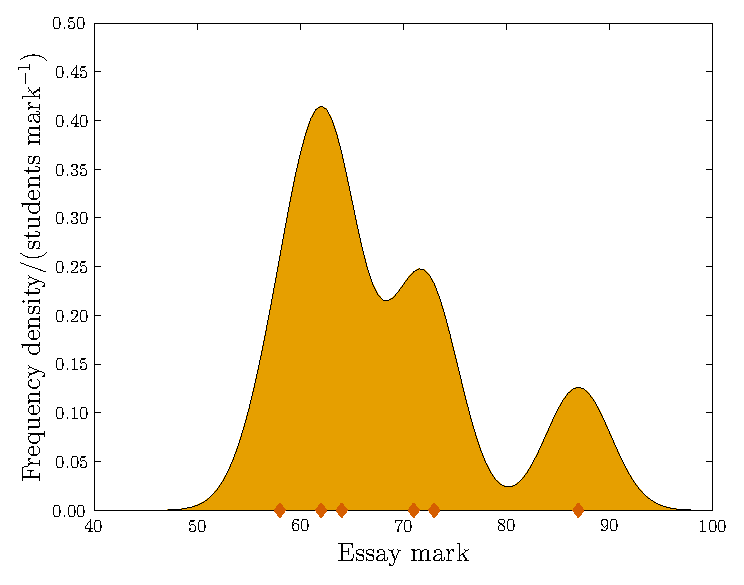
\includegraphics[width=0.47\textwidth]{./figs/Fig_2013_marks}} \quad
   \subfigure[{2014/2015}]{\label{fig:2014-marks} 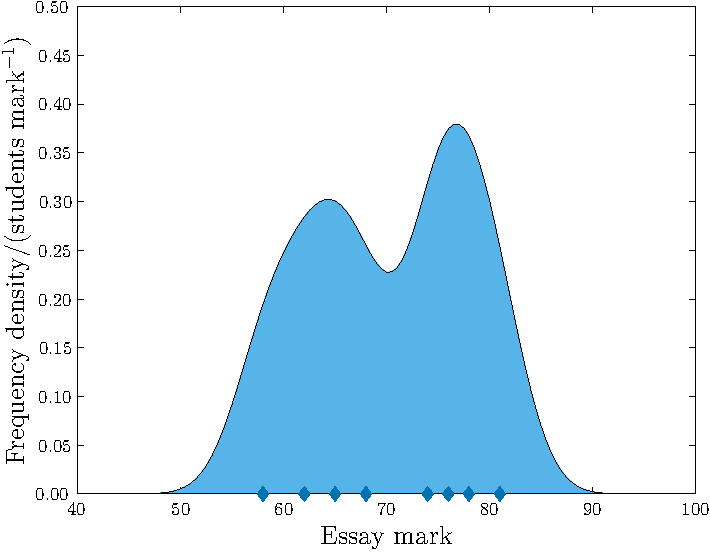
\includegraphics[width=0.47\textwidth]{./figs/Fig_2014_marks}}  
\caption{Distribution of essay marks for both cohorts of students. The diamonds indicate the actual marks; the frequency densities have been constructed by smoothing with a Gaussian kernel with a standard deviation of $\sqrt{10}~\mathrm{marks}$. The mean mark of the 2013/2014 students is $(68.1\pm3.4)~\mathrm{marks}$, and the mean for 2014/2015 students is $(70.3\pm2.7)~\mathrm{marks}$, where the uncertainties quoted on the means are estimated from the standard errors \citep[chapter 22]{Mackay2003}.}
  \label{fig:marks}
\end{figure}

Before we can draw conclusions from the distribution marks, it is necessary to consider the aptitudes of the students. Ideally, we would like to compare with marks from their first-year essays, to assess progress. I do not have access to these. However, I do have their average mark from first-year (a mark between $0$ and $100$). We would expect this to be correlated with their second-year essay mark. In \figref{diff}, we plot the distribution of differences between essay marks and their first-year averages.\footnote{Using relative difference instead of absolute difference gives qualitatively similar distributions.} We use the same Gaussian smoothing as in \figref{marks}. The 2013/2014 distribution shows a bimodal structure, with some students doing better than expected on their essay and others doing worse. The division is not related to tutorial group. There is no clear outlier (the high scoring student from \figref{2013-marks} has been absorbed into the better-than-expected peak). The 2014/2015 distribution is more consistent with expectations; the bimodality seen in \figref{marks} is an artefact of having two groups of different abilities.
\begin{figure}
  \centering
   \subfigure[{2013/2014}]{\label{fig:2013-diff} 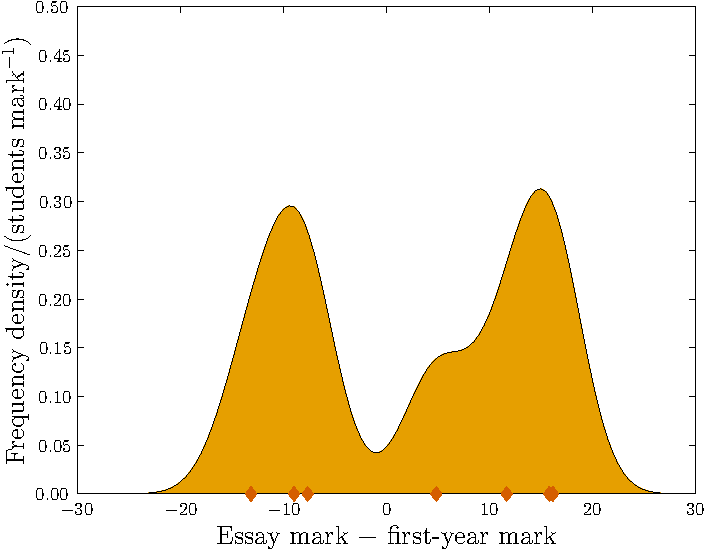
\includegraphics[width=0.47\textwidth]{./figs/Fig_2013_mark_diff}} \quad
   \subfigure[{2014/2015}]{\label{fig:2014-diif} 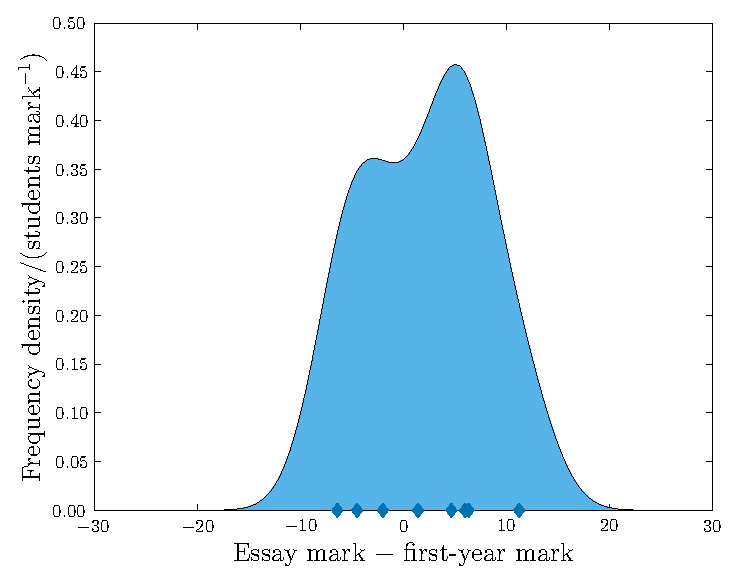
\includegraphics[width=0.47\textwidth]{./figs/Fig_2014_mark_diff}}  
\caption{Distribution of difference between essay and average first-year marks for both cohorts of students. The diamonds indicate the actual mark differences; the frequency densities have been constructed by smoothing with a Gaussian kernel with a standard deviation of $\sqrt{10}~\mathrm{marks}$. A positive difference indicates the student did better on the essay than in first year. The mean mark difference of the 2013/2014 students is $(2.7\pm4.3)~\mathrm{marks}$, and the mean for 2014/2015 students is $(2.1\pm2.0)~\mathrm{marks}$. Averaging across both cohorts, the mean mark difference is $(2.4\pm2.3)~\mathrm{marks}$. The uncertainties quoted on the means are estimated from the standard errors.}
  \label{fig:diff}
\end{figure}

The difference between the two years is striking, but we are dealing with small sample sizes. In 2013/2014 I had one student who took special interest in the essay, and another who took no interest in revision and so underperformed in exams; the factors can go some way towards accounting for the over-performance in the essay compared to first year. Equally, I had one student who misjudged the level of rigour needed in an essay and performed worse than I expected given their enthusiasm and scientific ability.\footnote{They resubmitted and their second mark was more consistent with their first-year mark. The difference after remarking was $-5~\mathrm{marks}$ and I suspect further that improvement would have been achieved if they were not conscious of the cap at $60~\mathrm{marks}$.} In 2014/2015 I had students who achieved higher marks in first-year, it is much more difficult for them to achieve a significantly higher mark in their essays, so one might expect the differences to taper off. Without a larger population of results, we must be cautious in drawing conclusions.

While it is possible to explain away differences, this does neglect the fact that there will always be a range of student abilities and motivations. Teaching must take this diversity into account. In \figref{mark-mark-diff}, we further examine the difference between the essay and first-year marks. In 2014/2015 there is no obvious correlation between the mark difference and performance in the essay, this is not the case in 2013/2014. Those who did well seem to show significant improvement compared to first year, while those who did badly show under-performance, although the two clusters overlap in terms of just essay mark. This is evidence of my 2013/2014 teaching having a polarising effect: those who were able to assimilate it went on to perform well, but those who were unable performed badly. In 2014/2015, my teaching of essay writing was more evenly distributed throughout the year (see \secref{essay-methods}), and involved a greater variety of methods, this may have made it more accessible and easier to digest, benefiting a greater selection of students. However, in distributing the teaching, it seems to have lost some of its impact, and there is not as great an increase in marks. Moving some of the discussion to the Autumn term, may have diluted the impact of giving advice while the essay was being written. It appears that there are potentially advantages and disadvantages to the adaptations I made to my teaching schedule.
\begin{figure}
  \centering
   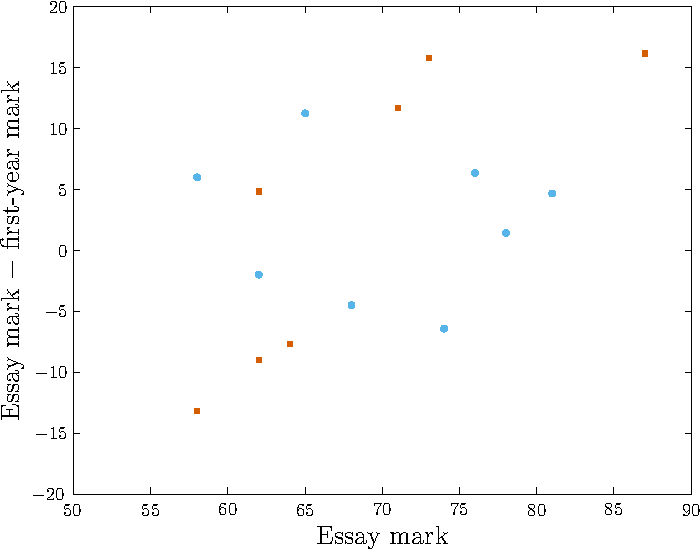
\includegraphics[width=0.6\textwidth]{./figs/Fig_mark_mark_diff}
\caption{Difference between essay and average first-year marks as a function of essay marks. The red--orange squares are the results for the 2013/2014 students and the light blue circles are for the 2014/2015 students. The 2013/2014 appear to fall into two clusters: those with positive mark differences and those with negative mark differences. The mean essay mark for the positive-difference group is $(73.3\pm4.5)~\mathrm{marks}$, and the mean for the negative-difference group is $(61.3\pm1.4)~\mathrm{marks}$, where the uncertainties quoted are estimated from the standard errors.}
  \label{fig:mark-mark-diff}
\end{figure}

There is one further statistic that can be incorporated into our analysis, tutorial attendance. We would expect attendance to be correlated with attainment. First, there is a causal link: those who spend more time engaging with educational activities should see a greater benefit from them. Second, attendance can be linked to motivation, which is correlated with learning \citep[e.g.,][chapter 4]{Ramsden1992}. Absence from tutorial could be because of apathy or disorganisation (see \secref{other-discuss}); because of poor health or personal matters, or because a clash with another educational activity such as an extracurricular or careers event. The first set of reasons indicates a lack of engagement with or low-prioritisation of their studies, which would be correlated with poor attainment. The second set does indicate anything about how the student views the subject or their studies, but may still be linked to a lack of motivation as as a side effect of potentially depressing problems. The final set may indicate that the student is positively engaged in their studies, taking an active interest in the subject or their own achievement; this may indicate good attainment, if this benefit outweighs the disadvantage of missing teaching sessions. In \figref{attend} we plot fractional attendance for year (the $20$ tutorials) against essay mark. There is no obvious correlation for 2013/2014, but there does appear to be the expected positive trend for 2014/2015.
\begin{figure}
  \centering
   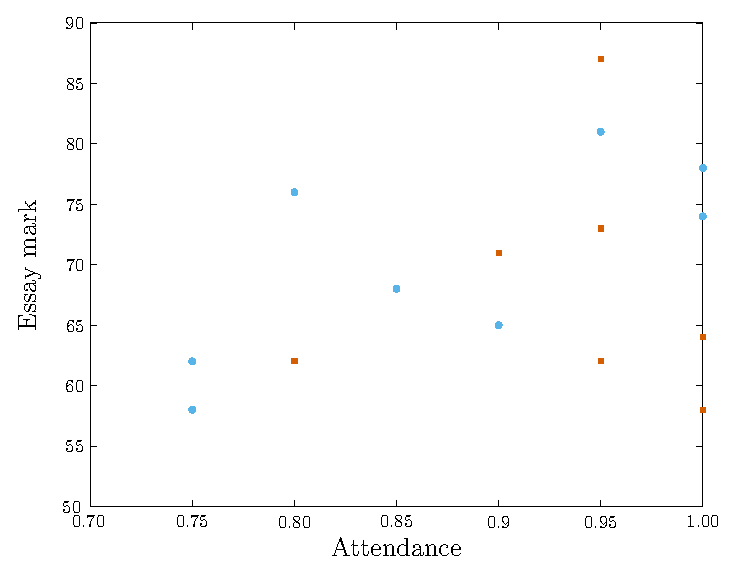
\includegraphics[width=0.6\textwidth]{./figs/Fig_attend}
\caption{Essay mark as a function of tutorial attendance. The red--orange squares are the results for the 2013/2014 students and the light blue circles are for the 2014/2015 students. There are $20$ tutorials, hence attendance is quantized into divisions on $0.05$.}
  \label{fig:attend}
\end{figure}

The difference between the cohorts could again be attributed to the small sample sizes; however, it may also trace the difference in teaching. In 2013/2014, teaching of essay writing was concentrated to tutorials 12 and 14 (see \tabref{2013-14}). Attendance at these two sessions was perfect. Hence no students suffered from missing an important lesson. The second-order effect of the impact of motivation (as traced by attendance) on performance appears to be negligible. In 2014/2015, teaching of communication skill was distributed throughout the year, making any given absence more significant. If we only consider the main essay-writing tutorials 3, 12, 13 and 14 (\tabref{2014-15}), the trend persists.  One student attended half of these tutorials and received an essay mark of $62~\mathrm{marks}$; two attended three out of four and received a mean mark of $(67.0\pm6.4)~\mathrm{marks}$, and the remaining five attended all four and have an mean mark of $(73.2\pm2.7)~\mathrm{marks}$. The quoted uncertainties on the means have been estimated from the standard error \citep[chapter 22]{Mackay2003}. Attendance appears to correlate with performance as being absent from tutorial means that students miss useful teaching. The provision of written materials, like a blog (\secref{blog}), that can be studied any time may ameliorate the impact of missing tutorial, but only if students are aware of there existence and importance. Breaking up teaching across multiple tutorials increases the probability that one or more sessions will be missed; however, it also reduces the probability that all of the teaching on essay-writing is missed, which would likely be extremely detrimental.

\section{Summary \& conclusion}\label{sec:marks-end}

From the limited data available, we may draw some provisional qualitative conclusions on the effectiveness of teaching. Making more robust statements would require a more sophisticated analysis or further data. Unsurprisingly, our data suggest that essay-writing ability is correlated both with overall proficiency (measured by average first-year mark) and attendance at tutorials where essay-writing was discussed. Comparing the two cohorts, it appears that the more distributed teaching of 2014/2015 is safer. Students are less likely to under-perform and there is a lower risk of missing all the relevant teaching. However, the teaching of 2013/2014 was more effective at inspiring significant over-performance (compared to the first-year mark). This may be because a concentrated session during the Spring term is particularly effective, as students can immediately make use of the information, but we do not have the evidence to prove this. We conclude, that neither the teaching of 2013/2014 nor 2014/2015 is superior to the other in all regards.


\backmatter

\phantomsection
\bookmarksetup{startatroot}

\bibliographystyle{../physicsAuthorYearURL2}
\addcontentsline{toc}{chapter}{References}
\bibliography{../teaching}

\end{document}
